
\subsection{Explotar o seguir explorando}\label{subsection:exp-epsilon}

En esta sección se muestran los experimentos para comparar
el desempeño de los algoritmos con dos valores diferentes para
el factor que controla la tasa de decremento de $\epsilon$. El primer valor 
es bajo, para dejar de dar peso a la exploración después del primer
cuarto de entrenamiento y el segundo es alto, para llegar a una máxima probabilidad
de explotación en el último cuarto del aprendizaje.

\subsubsection{Configuración experimental}

\begin{itemize}
    \item El espacio de estados es discreto, es decir, el agente puede
    obtener las variables $\mathcal{X}$ directamente del ambiente.
    \item Para obtener a los
    grafos $\mathcal{D'}$ y $\mathcal{D''}$,
    el porcentaje de nivel de cambio  es $p_{mod} = 25 \%$. Esto significa que no se altera demasiado el grafo causal original para
    generar los grafos incompletos e incorrectos.
    \item Se controla qué tan rápido se desea alcanzar $\epsilon_{\min}$ variando el parámetro $\delta$. Si se divide al entrenamiento en cuartos,  entonces los valores de $\delta$ corresponden a en qué cuarto se alcanza el mínimo valor para $\epsilon$.
    \begin{itemize}
        \item Alcanzar $\epsilon_{\min}$ en el primer cuarto del entrenamiento, $\delta = 0.25$.
        \item Alcanzar $\epsilon_{\min}$ a medio aprendizaje, $\delta = 0.50$.
        \item Alcanzar $\epsilon_{\min}$ en el tercer cuarto del entrenamiento, $\delta = 0.75$.
    \end{itemize}
    \item Se examina sobre los tres tipos de estructuras posibles: uno-a-uno, 
    causa común y efecto común. 
    \item Se prueba sobre un mundo determinista y estocástico.
    \item Dado que en la sección \ref{exp1}, $\delta=0.5$, este valor se deja fuera para estos experimentos.
\end{itemize}

\subsubsection{Objetivo}

Determinar si reducir o aumentar las consultas al grafo causal a lo largo del aprendizaje afecta el desempeño
de los algoritmos.

\subsubsection{Hipótesis}

La información del grafo causal no afecta negativamente 
el aprendizaje de la función de valor $Q$. Por lo tanto, incluso si se disminuyen las consultas al modelo de manera temprana en el entrenamiento, la información provista habrá
ayudado al aprendizaje de la función de valor.

\subsubsection{Resultados}

En las Figuras \ref{fig:low-epsilon-det} y \ref{fig:high-epsilon-det} se puede ver que los algoritmos que utilizan conocimiento del grafo inician con una recompensa mayor y se estabilizan más rápido que el algoritmo Q-learning
sin información adicional en ambientes con transiciones deterministas y estocásticas.
De acuerdo con los resultados parece que 
entre mayor sea $\delta$ más tarda en estabilizarse
el algoritmo de aprendizaje sin información que lo auxilie. Esto es de esperarse, ya que se sigue explorando durante más tiempo. 
% Sin embargo,
% también se puede notar que estimula a dejar
% la exploración de manera temprana, no implica que después
% de dejarla, el algoritmo converge inmediatamente. 
Por otro lado, para las estructuras uno-a-uno, la recompensa en los algoritmos que se guían por el grafo, se desestabiliza el intervalo en el que se encuentra la transición a dejar de dar peso a
la exploración. Pero, una vez fuera de esa ``zona de transición'' los
algoritmos se recuperan y tienden a estar por encima del algoritmo sin datos 
extra.

\newpage

% Please add the following required packages to your document preamble:
% \usepackage{booktabs}
% \usepackage{graphicx}
\begin{table}[]
\centering
\caption{Uno a uno}
\label{tab:delta-one-to-one}
\resizebox{\textwidth}{!}{%
\begin{tabular}{@{}ccclll@{}}
\toprule
Ambiente & $\delta$ & Algoritmo & \multicolumn{3}{c}{$N$} \\ \cmidrule(l){4-6} 
 &  &  & \multicolumn{1}{c}{5} & \multicolumn{1}{c}{7} & \multicolumn{1}{c}{9} \\ \midrule
Determinista & $0.25$ & $Q_{1}$ & $-2.2324 \pm 0.6353$ & $-4.3184 \pm 0.8746$ & $-6.3564 \pm 1.3603$ \\
 &  & $Q_{2}$ & $\mathbf{-1.9466 \pm 0.4679}$ & $-3.5731 \pm 0.7285$ & $-5.7115 \pm 1.1855$ \\
 &  & $Q_{2}$ & $-1.9825 \pm 0.4632$ & $\mathbf{-3.5061 \pm 0.7207}$ & $\mathbf{-5.6209 \pm 1.0718}$ \\
 &  & $Q_{4}$ & $-2.0330 \pm 0.5384$ & $-3.5547 \pm 0.7081$ & $-5.8372 \pm 1.0747$ \\ \cmidrule(l){2-6} 
 & $0.75$ & $Q_{1}$ & $-2.3774 \pm 0.6925$ & $-4.3218 \pm 0.9312$ & $-6.2775 \pm 1.1195$ \\
 &  & $Q_{2}$ & $\mathbf{-1.8880 \pm 0.4666}$ & $\mathbf{-3.4929 \pm 0.7115}$ & $-6.9414 \pm 1.6493$ \\
 &  & $Q_{2}$ & $-2.1314 \pm 0.4933$ & $-3.8299 \pm 0.7694$ & $-6.3671 \pm 1.4099\dagger$ \\
 &  & $Q_{4}$ & $-1.9896 \pm 0.5470$ & $-3.8252 \pm 0.7840$ & $\mathbf{-6.2538 \pm 1.3547\dagger}$ \\ \cmidrule(l){2-6} 
Estocástico & $0.25$ & $Q_{1}$ & $-4.8575 \pm 0.9453$ & $-9.3174 \pm 1.2780$ & $-14.5087 \pm 1.4934$ \\
 &  & $Q_{2}$ & $\mathbf{-3.4833 \pm 0.8100}$ & $-7.2904 \pm 1.3719$ & $\mathbf{-10.7682 \pm 1.8282}$ \\
 &  & $Q_{2}$ & $-3.7870 \pm 0.8263$ & $\mathbf{-6.8757 \pm 1.2246}$ & $-11.9817 \pm 1.9420$ \\
 &  & $Q_{4}$ & $-3.8850 \pm 0.8119$ & $-7.1184 \pm 1.1471$ & $-12.4496 \pm 1.9692$ \\ \cmidrule(l){2-6} 
 & $0.75$ & $Q_{1}$ & $-5.0956 \pm 0.8950$ & $-9.3535 \pm 1.2484$ & $-14.3432 \pm 1.7236$ \\
 &  & $Q_{2}$ & $\mathbf{-3.9598 \pm 0.8291}$ & $-8.1395 \pm 1.3979$ & $\mathbf{-13.7784 \pm 1.8453}$ \\
 &  & $Q_{2}$ & $-4.2412 \pm 0.9166$ & $-8.4381 \pm 1.4981$ & $-13.8170 \pm 2.0379\dagger$ \\
 &  & $Q_{4}$ & $-3.9809 \pm 0.8148$ & $\mathbf{-8.1071 \pm 1.2102}$ & $-13.9492 \pm 1.7832\dagger$ \\ \bottomrule
\end{tabular}%
}
\end{table}

\begin{table}[]
\centering
\caption{Causa común}
\label{tab:delta-one-to-many}
\resizebox{\textwidth}{!}{%
\begin{tabular}{@{}ccclll@{}}
\toprule
Ambiente & $\delta$ & Algoritmo & \multicolumn{3}{c}{$N$} \\ \cmidrule(l){4-6} 
 &  &  & \multicolumn{1}{c}{5} & \multicolumn{1}{c}{7} & \multicolumn{1}{c}{9} \\ \midrule
Determinista & $0.25$ & $Q_{1}$ & $-2.2324 \pm 0.6353$ & $-4.3184 \pm 0.8746$ & $-6.3564 \pm 1.3603$ \\
 &  & $Q_{2}$ & $\mathbf{-1.9466 \pm 0.4679}$ & $-3.5731 \pm 0.7285$ & $-5.7115 \pm 1.1855$ \\
 &  & $Q_{2}$ & $-1.9825 \pm 0.4632$ & $\mathbf{-3.5061 \pm 0.7207}$ & $\mathbf{-5.6209 \pm 1.0718}$ \\
 &  & $Q_{4}$ & $-2.0330 \pm 0.5384$ & $-3.5547 \pm 0.7081$ & $-5.8372 \pm 1.0747$ \\ \cmidrule(l){2-6} 
 & $0.75$ & $Q_{1}$ & $-2.3774 \pm 0.6925$ & $-4.3218 \pm 0.9312$ & $-6.2775 \pm 1.1195$ \\
 &  & $Q_{2}$ & $\mathbf{-1.8880 \pm 0.4666}$ & $\mathbf{-3.4929 \pm 0.7115}$ & $-6.9414 \pm 1.6493$ \\
 &  & $Q_{2}$ & $-2.1314 \pm 0.4933$ & $-3.8299 \pm 0.7694$ & $-6.3671 \pm 1.4099\dagger$ \\
 &  & $Q_{4}$ & $-1.9896 \pm 0.5470$ & $-3.8252 \pm 0.7840$ & $\mathbf{-6.2538 \pm 1.3547\dagger}$ \\ \cmidrule(l){2-6} 
Estocástico & $0.25$ & $Q_{1}$ & $-4.8575 \pm 0.9453$ & $-9.3174 \pm 1.2780$ & $-14.5087 \pm 1.4934$ \\
 &  & $Q_{2}$ & $\mathbf{-3.4833 \pm 0.8100}$ & $-7.2904 \pm 1.3719$ & $\mathbf{-10.7682 \pm 1.8282}$ \\
 &  & $Q_{2}$ & $-3.7870 \pm 0.8263$ & $\mathbf{-6.8757 \pm 1.2246}$ & $-11.9817 \pm 1.9420$ \\
 &  & $Q_{4}$ & $-3.8850 \pm 0.8119$ & $-7.1184 \pm 1.1471$ & $-12.4496 \pm 1.9692$ \\ \cmidrule(l){2-6} 
 & $0.75$ & $Q_{1}$ & $-5.0956 \pm 0.8950$ & $-9.3535 \pm 1.2484$ & $-14.3432 \pm 1.7236$ \\
 &  & $Q_{2}$ & $\mathbf{-3.9598 \pm 0.8291}$ & $-8.1395 \pm 1.3979$ & $\mathbf{-13.7784 \pm 1.8453}$ \\
 &  & $Q_{2}$ & $-4.2412 \pm 0.9166$ & $-8.4381 \pm 1.4981$ & $-13.8170 \pm 2.0379\dagger$ \\
 &  & $Q_{4}$ & $-3.9809 \pm 0.8148$ & $\mathbf{-8.1071 \pm 1.2102}$ & $-13.9492 \pm 1.7832\dagger$ \\ \bottomrule
\end{tabular}%
}
\end{table}

\begin{table}[]
\centering
\caption{Efecto común}
\label{tab:delta-many-to-one}
\resizebox{\textwidth}{!}{%
\begin{tabular}{@{}ccclll@{}}
\toprule
Ambiente & $\delta$ & Algoritmo & \multicolumn{3}{c}{$N$} \\ \cmidrule(l){4-6} 
 &  &  & \multicolumn{1}{c}{5} & \multicolumn{1}{c}{7} & \multicolumn{1}{c}{9} \\ \midrule
Determinista & $0.25$ & $Q_{1}$ & $-2.2324 \pm 0.6353$ & $-4.3184 \pm 0.8746$ & $-6.3564 \pm 1.3603$ \\
 &  & $Q_{2}$ & $\mathbf{-1.9466 \pm 0.4679}$ & $-3.5731 \pm 0.7285$ & $-5.7115 \pm 1.1855$ \\
 &  & $Q_{2}$ & $-1.9825 \pm 0.4632$ & $\mathbf{-3.5061 \pm 0.7207}$ & $\mathbf{-5.6209 \pm 1.0718}$ \\
 &  & $Q_{4}$ & $-2.0330 \pm 0.5384$ & $-3.5547 \pm 0.7081$ & $-5.8372 \pm 1.0747$ \\ \cmidrule(l){2-6} 
 & $0.75$ & $Q_{1}$ & $-2.3774 \pm 0.6925$ & $-4.3218 \pm 0.9312$ & $-6.2775 \pm 1.1195$ \\
 &  & $Q_{2}$ & $\mathbf{-1.8880 \pm 0.4666}$ & $\mathbf{-3.4929 \pm 0.7115}$ & $-6.9414 \pm 1.6493$ \\
 &  & $Q_{2}$ & $-2.1314 \pm 0.4933$ & $-3.8299 \pm 0.7694$ & $-6.3671 \pm 1.4099\dagger$ \\
 &  & $Q_{4}$ & $-1.9896 \pm 0.5470$ & $-3.8252 \pm 0.7840$ & $\mathbf{-6.2538 \pm 1.3547\dagger}$ \\ \cmidrule(l){2-6} 
Estocástico & $0.25$ & $Q_{1}$ & $-4.8575 \pm 0.9453$ & $-9.3174 \pm 1.2780$ & $-14.5087 \pm 1.4934$ \\
 &  & $Q_{2}$ & $\mathbf{-3.4833 \pm 0.8100}$ & $-7.2904 \pm 1.3719$ & $\mathbf{-10.7682 \pm 1.8282}$ \\
 &  & $Q_{2}$ & $-3.7870 \pm 0.8263$ & $\mathbf{-6.8757 \pm 1.2246}$ & $-11.9817 \pm 1.9420$ \\
 &  & $Q_{4}$ & $-3.8850 \pm 0.8119$ & $-7.1184 \pm 1.1471$ & $-12.4496 \pm 1.9692$ \\ \cmidrule(l){2-6} 
 & $0.75$ & $Q_{1}$ & $-5.0956 \pm 0.8950$ & $-9.3535 \pm 1.2484$ & $-14.3432 \pm 1.7236$ \\
 &  & $Q_{2}$ & $\mathbf{-3.9598 \pm 0.8291}$ & $-8.1395 \pm 1.3979$ & $\mathbf{-13.7784 \pm 1.8453}$ \\
 &  & $Q_{2}$ & $-4.2412 \pm 0.9166$ & $-8.4381 \pm 1.4981$ & $-13.8170 \pm 2.0379\dagger$ \\
 &  & $Q_{4}$ & $-3.9809 \pm 0.8148$ & $\mathbf{-8.1071 \pm 1.2102}$ & $-13.9492 \pm 1.7832\dagger$ \\ \bottomrule
\end{tabular}%
}
\end{table}

\begin{figure}
\settoheight{\tempdima}{\includegraphics[width=.32\linewidth]{example-image-a}}%
\centering\begin{tabular}{@{}c@{ }c@{ }c@{ }c@{}}
&\textbf{Uno-a-uno} & \textbf{Causa común} & \textbf{Efecto común} \\
\rowname{$N = 5$}&
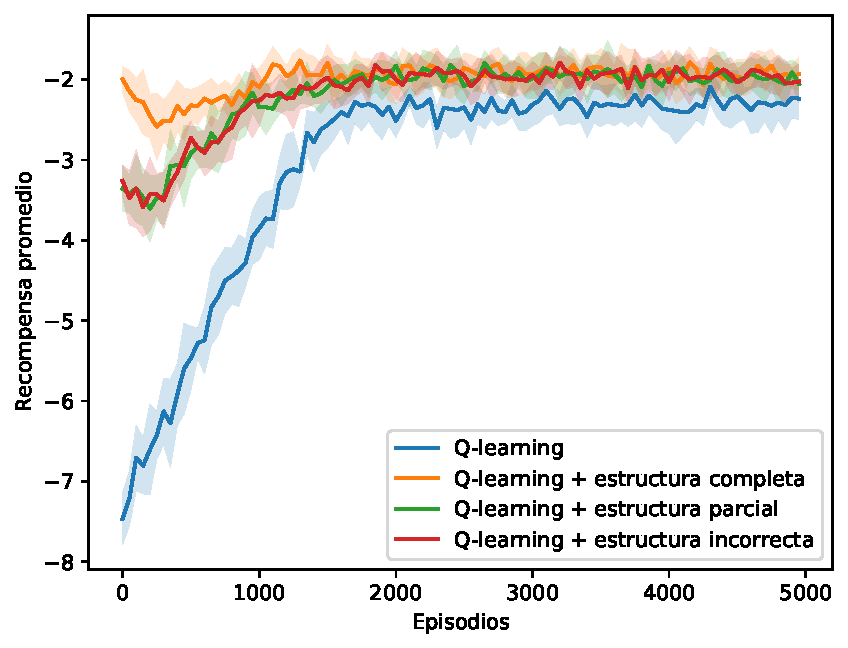
\includegraphics[width=.32\linewidth]{Chapter5/Figs/deltaexp/deterministic_low_025_one_to_one_N_5_experiments_10_episodes_5000_eps_6250.pdf}&
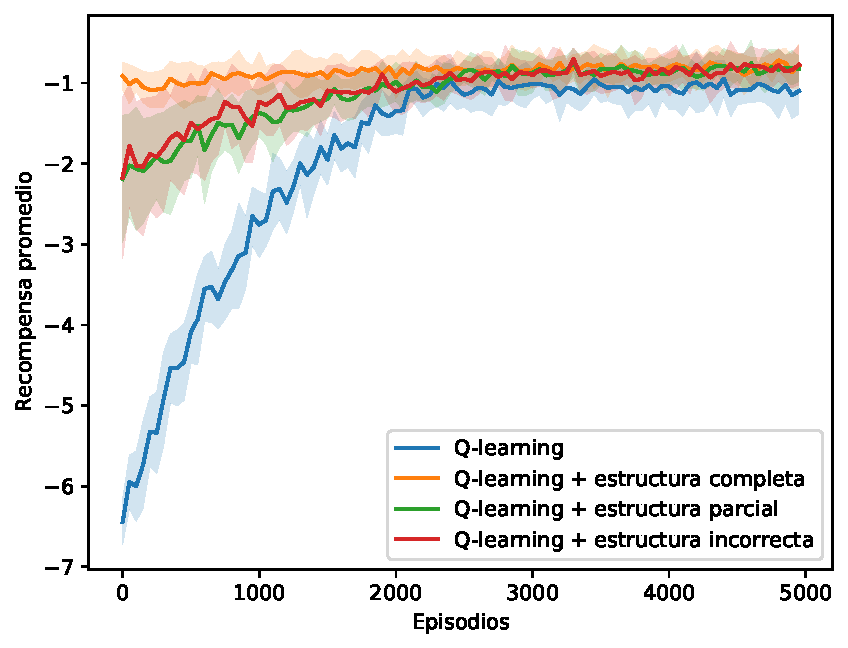
\includegraphics[width=.32\linewidth]{Chapter5/Figs/deltaexp/deterministic_low_025_one_to_many_N_5_experiments_10_episodes_5000_eps_6250.pdf}&
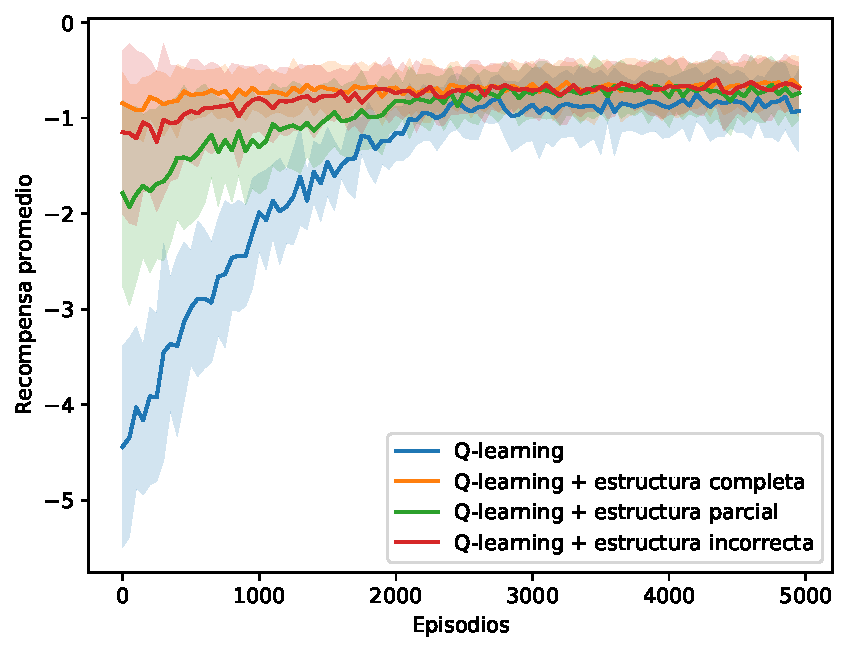
\includegraphics[width=.32\linewidth]{Chapter5/Figs/deltaexp/deterministic_low_025_many_to_one_N_5_experiments_10_episodes_5000_eps_6250.pdf}\\
\rowname{$N=7$}&
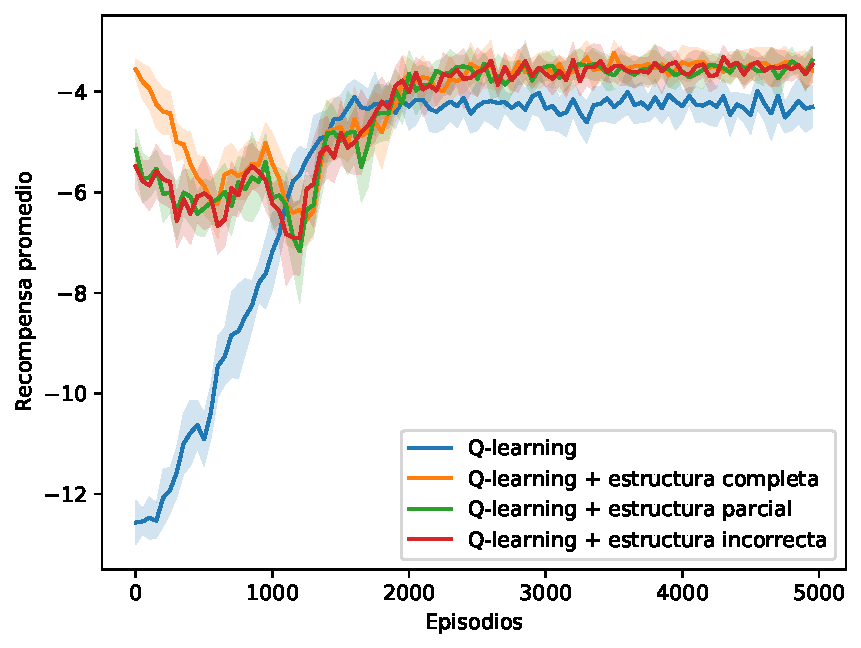
\includegraphics[width=.32\linewidth]{Chapter5/Figs/deltaexp/deterministic_low_025_one_to_one_N_7_experiments_10_episodes_5000_eps_8750.pdf}&
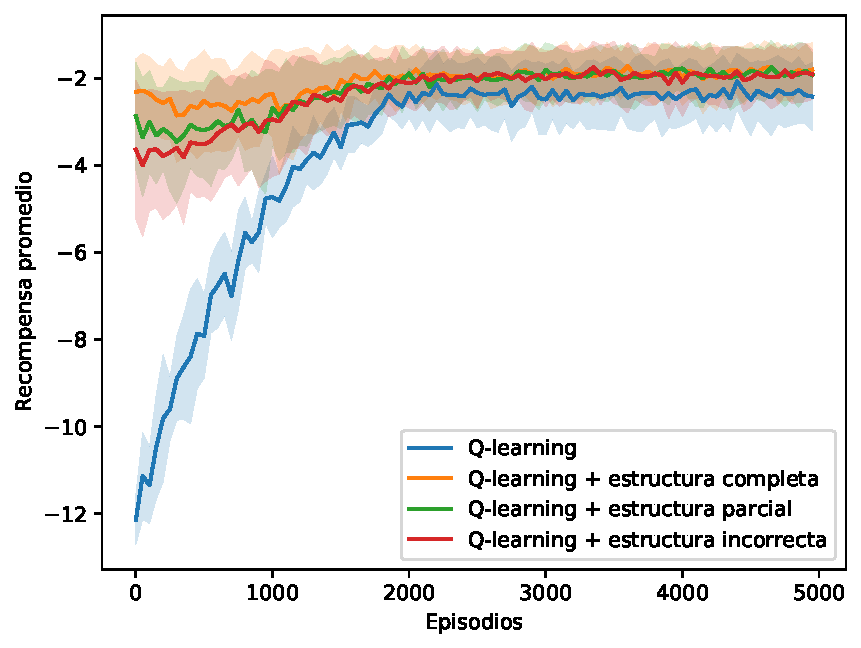
\includegraphics[width=.32\linewidth]{Chapter5/Figs/deltaexp/deterministic_low_025_one_to_many_N_7_experiments_10_episodes_5000_eps_8750.pdf}&
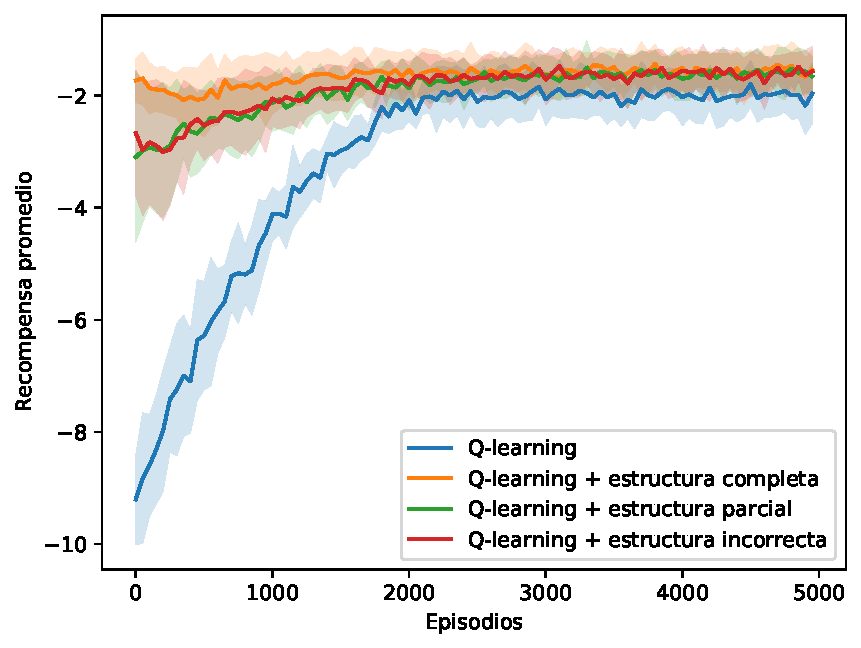
\includegraphics[width=.32\linewidth]{Chapter5/Figs/deltaexp/deterministic_low_025_many_to_one_N_7_experiments_10_episodes_5000_eps_8750.pdf}\\
\rowname{$N = 9$}&
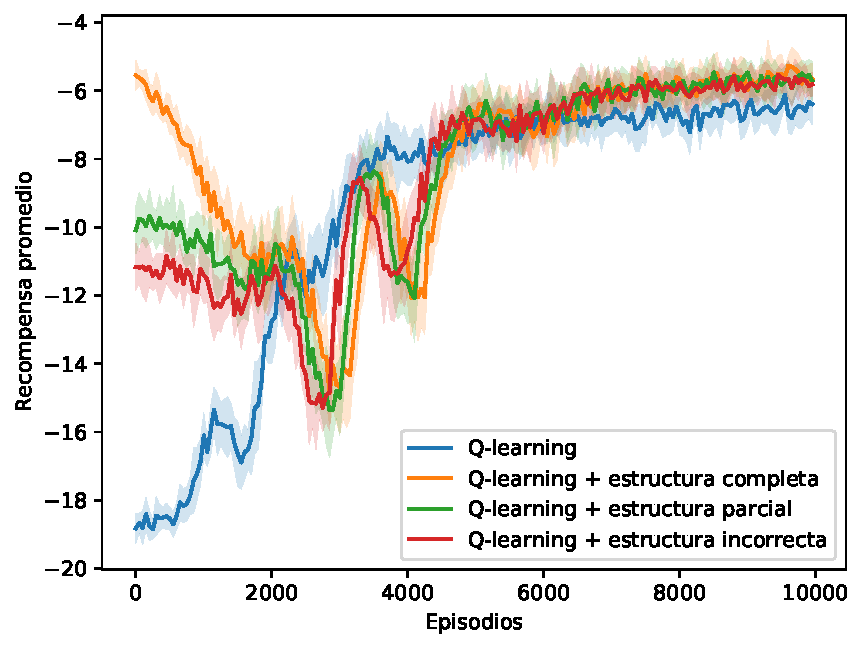
\includegraphics[width=.32\linewidth]{Chapter5/Figs/deltaexp/deterministic_low_025_one_to_one_N_9_experiments_10_episodes_10000_eps_22500.pdf}&
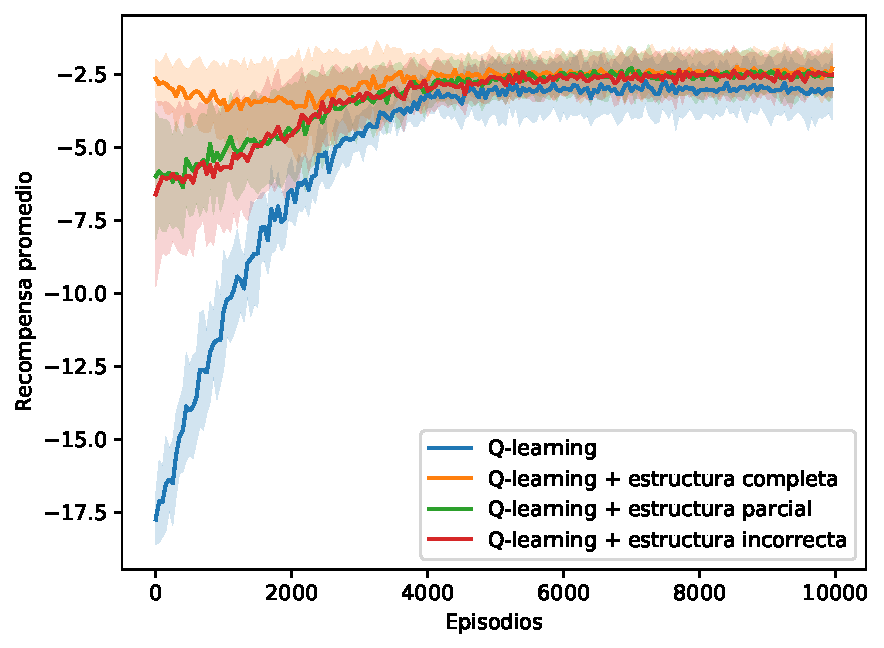
\includegraphics[width=.32\linewidth]{Chapter5/Figs/deltaexp/deterministic_low_025_one_to_many_N_9_experiments_10_episodes_10000_eps_22500.pdf}&
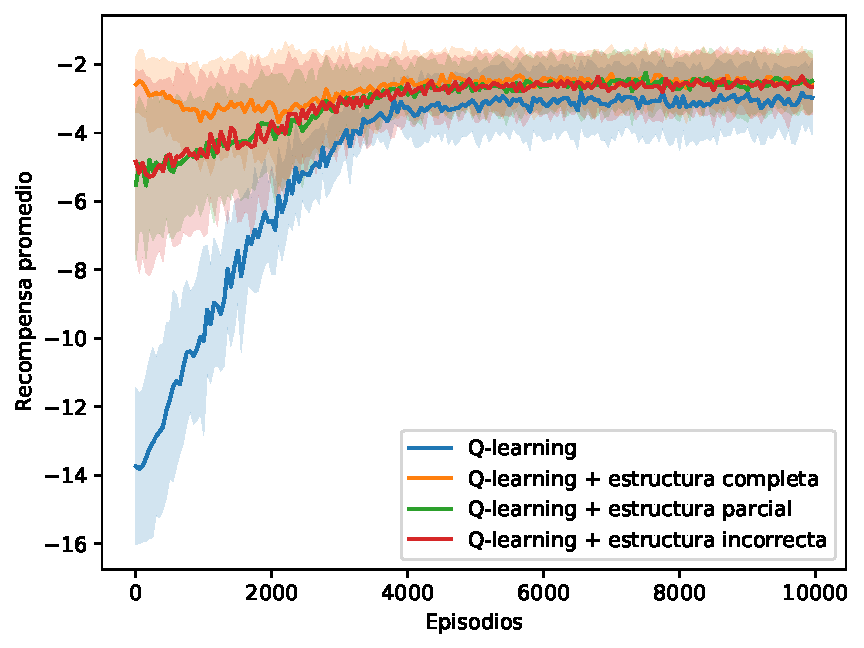
\includegraphics[width=.32\linewidth]{Chapter5/Figs/deltaexp/deterministic_low_025_many_to_one_N_9_experiments_10_episodes_10000_eps_22500.pdf}
\end{tabular}
\caption{Comparación del desempeño para los 4 algoritmos con un nivel de alteración $p_{mod} = 25 \%$  y $\delta = 0.25$ en un ambiente determinista. Las gráficas muestran la medida $average$ y la desviación estándar (región sombreada) para 10 experimentos con 5000 (para $N = 5, 7$) y 10000 (para $N = 9$) episodios.}
\label{fig:low-epsilon-det}
\end{figure}


\begin{figure}
\settoheight{\tempdima}{\includegraphics[width=.32\linewidth]{example-image-a}}%
\centering\begin{tabular}{@{}c@{ }c@{ }c@{ }c@{}}
&\textbf{Uno-a-uno} & \textbf{Causa común} & \textbf{Efecto común} \\
\rowname{$N = 5$}&
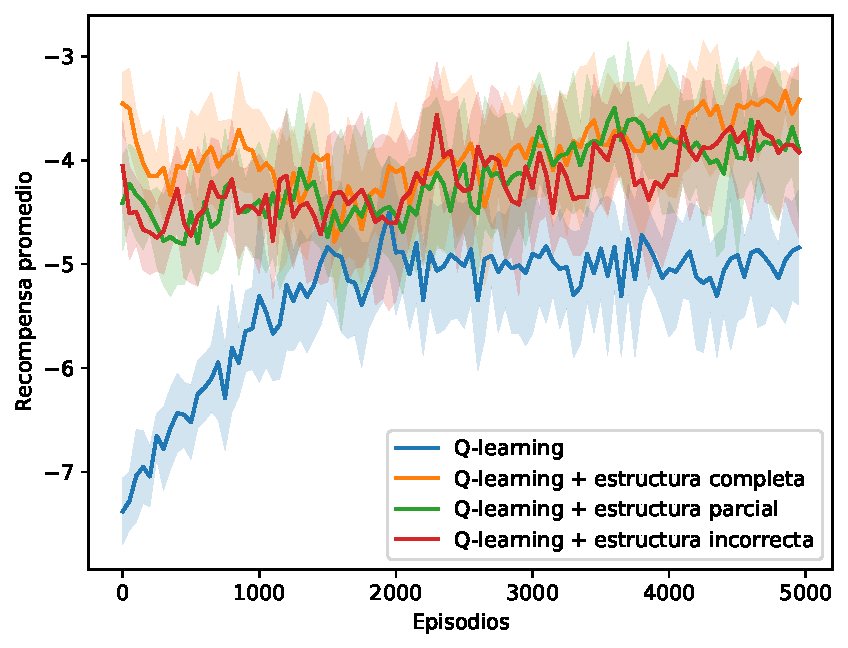
\includegraphics[width=.32\linewidth]{Chapter5/Figs/deltaexp/stochastic_low_025_one_to_one_N_5_experiments_10_episodes_5000_eps_6250.pdf}&
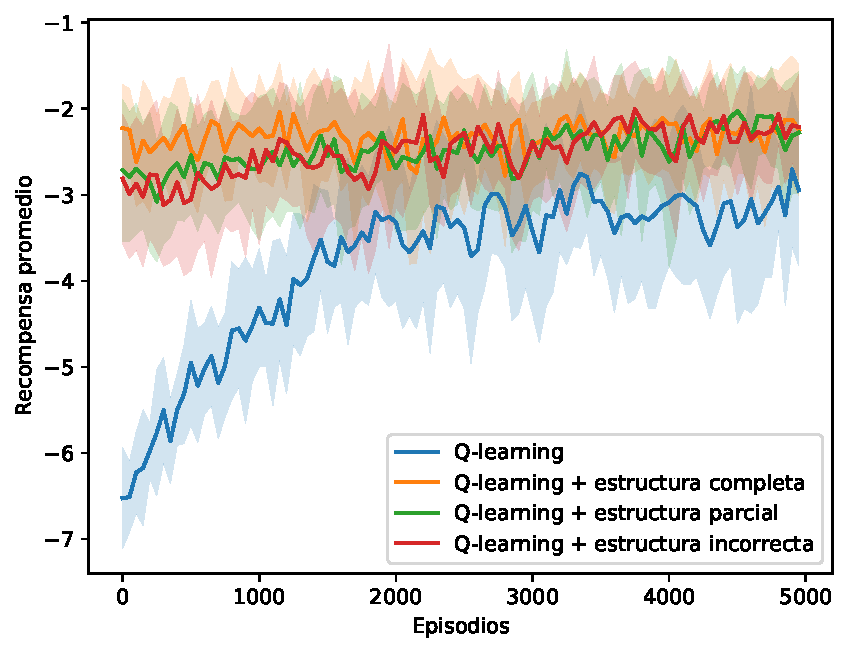
\includegraphics[width=.32\linewidth]{Chapter5/Figs/deltaexp/stochastic_low_025_one_to_many_N_5_experiments_10_episodes_5000_eps_6250.pdf}&
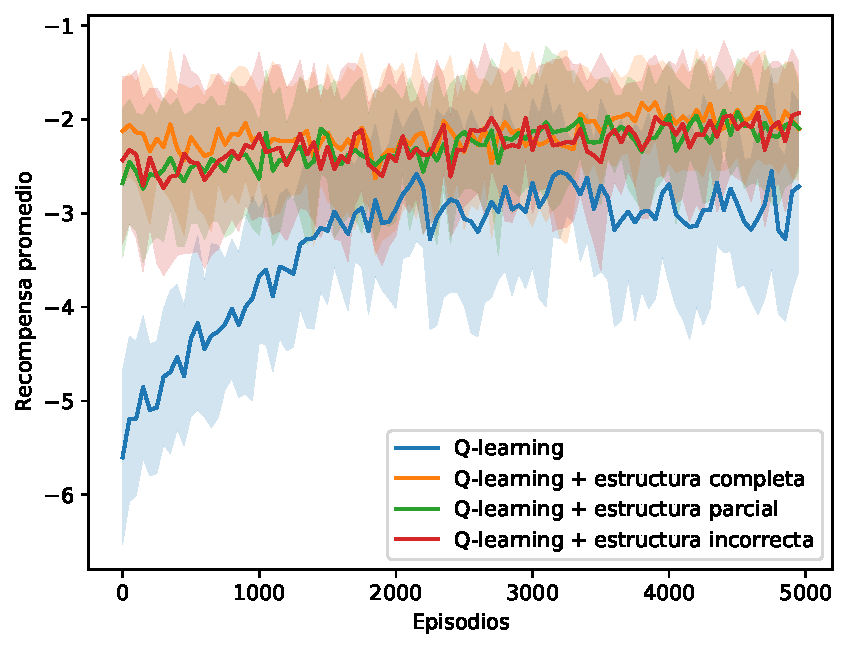
\includegraphics[width=.32\linewidth]{Chapter5/Figs/deltaexp/stochastic_low_025_many_to_one_N_5_experiments_10_episodes_5000_eps_6250.pdf}\\
\rowname{$N=7$}&
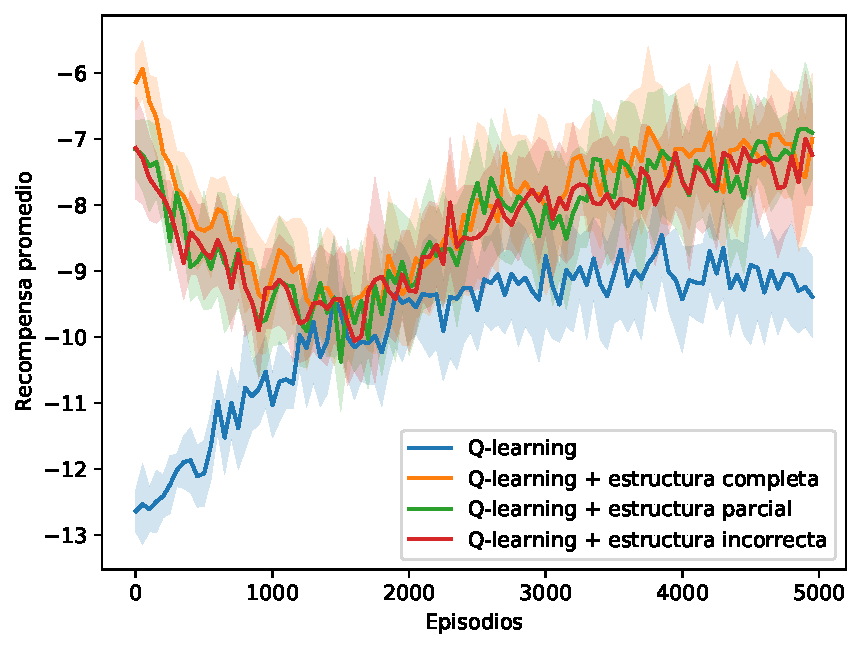
\includegraphics[width=.32\linewidth]{Chapter5/Figs/deltaexp/stochastic_low_025_one_to_one_N_7_experiments_10_episodes_5000_eps_8750.pdf}&
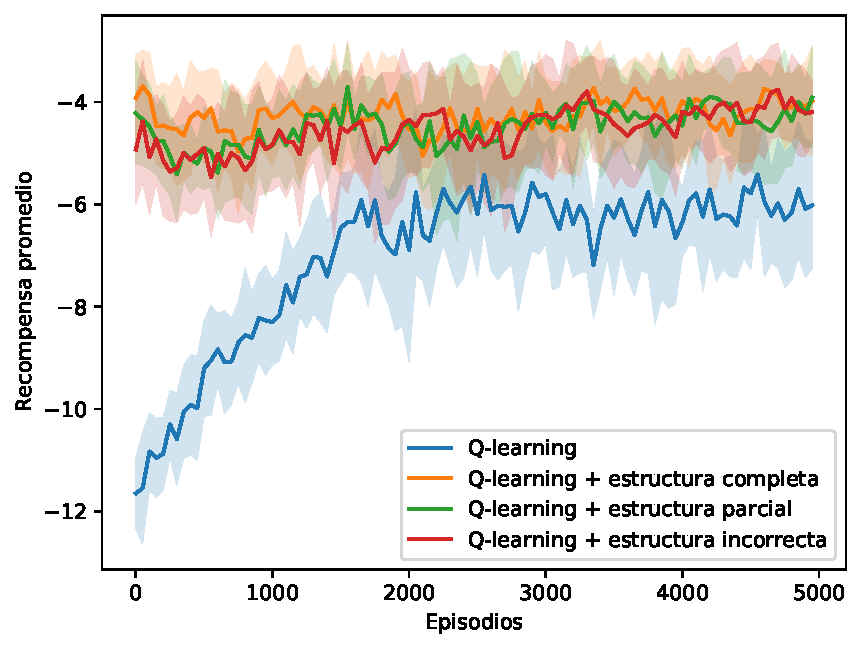
\includegraphics[width=.32\linewidth]{Chapter5/Figs/deltaexp/stochastic_low_025_one_to_many_N_7_experiments_10_episodes_5000_eps_8750.pdf}&
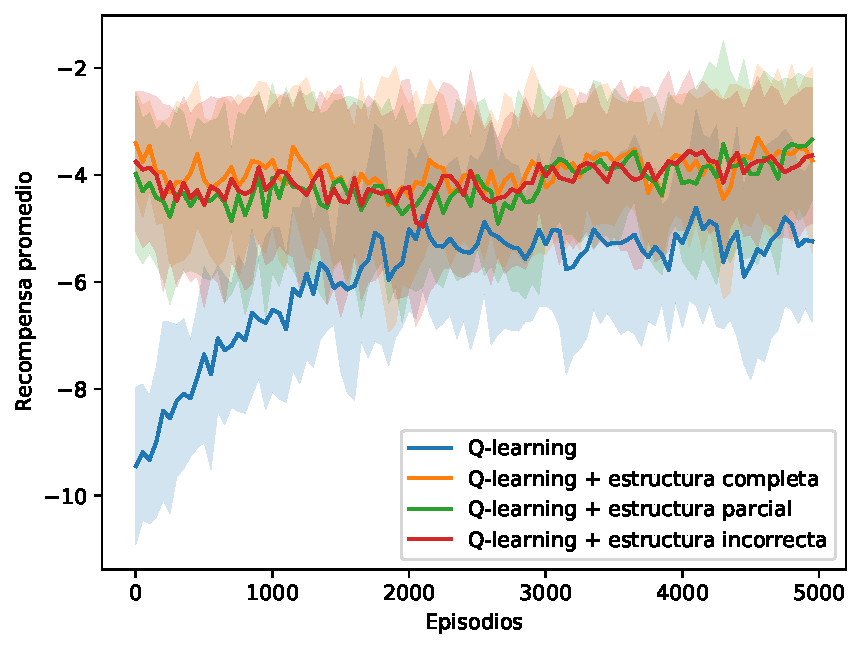
\includegraphics[width=.32\linewidth]{Chapter5/Figs/deltaexp/stochastic_low_025_many_to_one_N_7_experiments_10_episodes_5000_eps_8750.pdf}\\
\rowname{$N = 9$}&
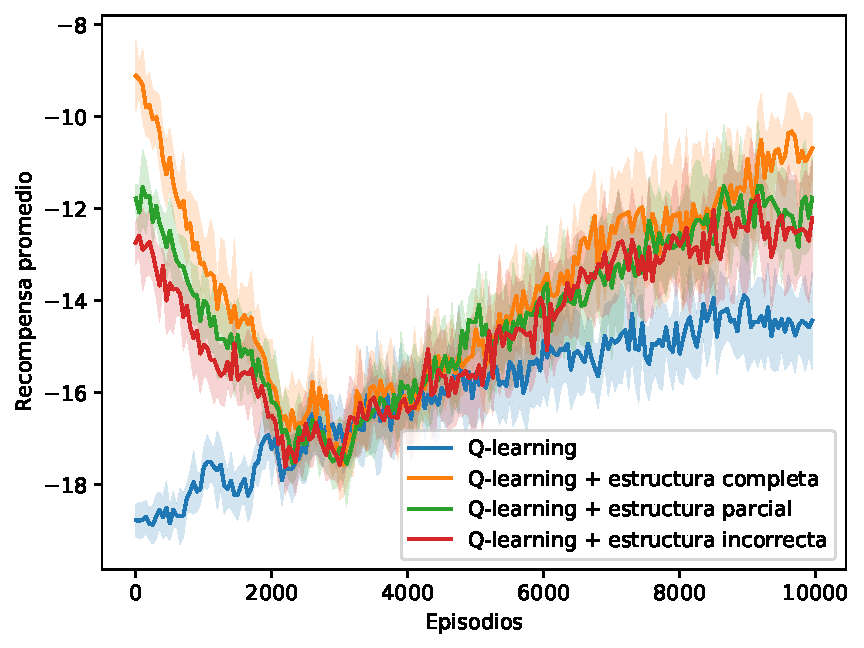
\includegraphics[width=.32\linewidth]{Chapter5/Figs/deltaexp/stochastic_low_025_one_to_one_N_9_experiments_10_episodes_10000_eps_22500.pdf}&
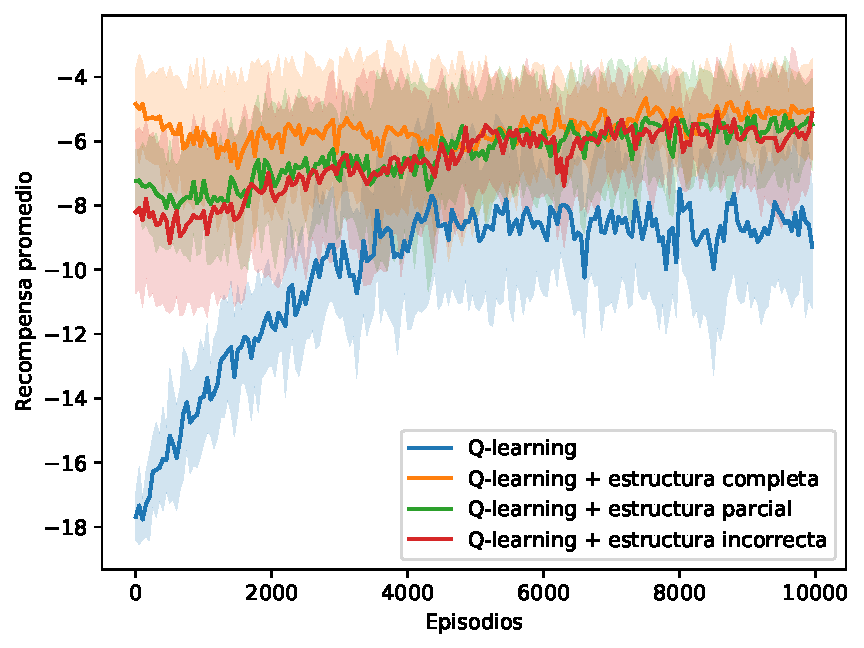
\includegraphics[width=.32\linewidth]{Chapter5/Figs/deltaexp/stochastic_low_025_one_to_many_N_9_experiments_10_episodes_10000_eps_22500.pdf}&
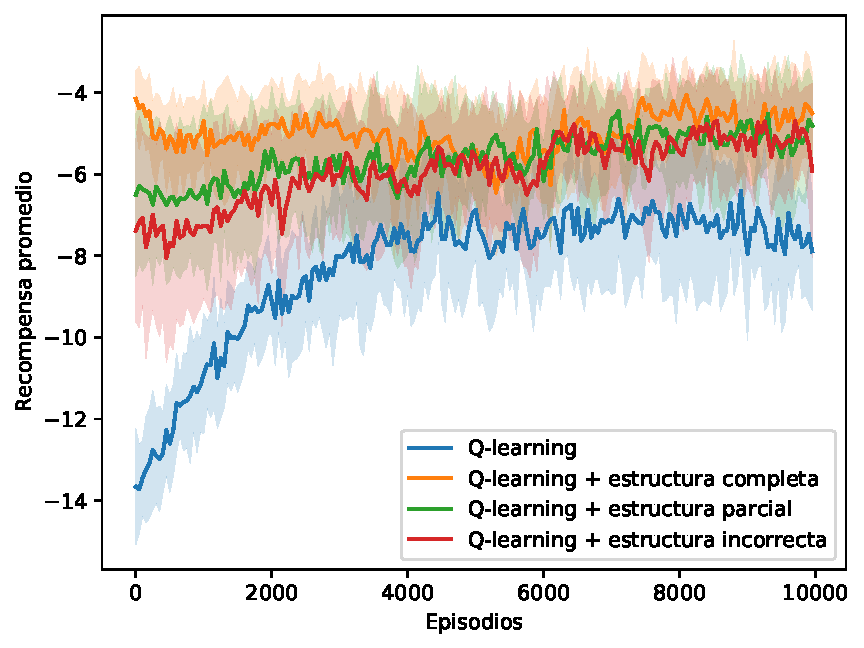
\includegraphics[width=.32\linewidth]{Chapter5/Figs/deltaexp/stochastic_low_025_many_to_one_N_9_experiments_10_episodes_10000_eps_22500.pdf}
\end{tabular}
\caption{Comparación del desempeño para los 4 algoritmos con un nivel de alteración $p_{mod} = 25 \%$  y $\delta = 0.25$ en un ambiente con transiciones estocásticas. Las gráficas muestran la medida $average$ y la desviación estándar (región sombreada)  para 10 experimentos con 5000 (para $N = 5, 7$) y 10000 (para $N = 9$) episodios.}
\label{fig:low-epsilon-sto}
\end{figure}



\begin{figure}
\settoheight{\tempdima}{\includegraphics[width=.32\linewidth]{example-image-a}}%
\centering\begin{tabular}{@{}c@{ }c@{ }c@{ }c@{}}
&\textbf{Uno-a-uno} & \textbf{Causa común} & \textbf{Efecto común} \\
\rowname{$N = 5$}&
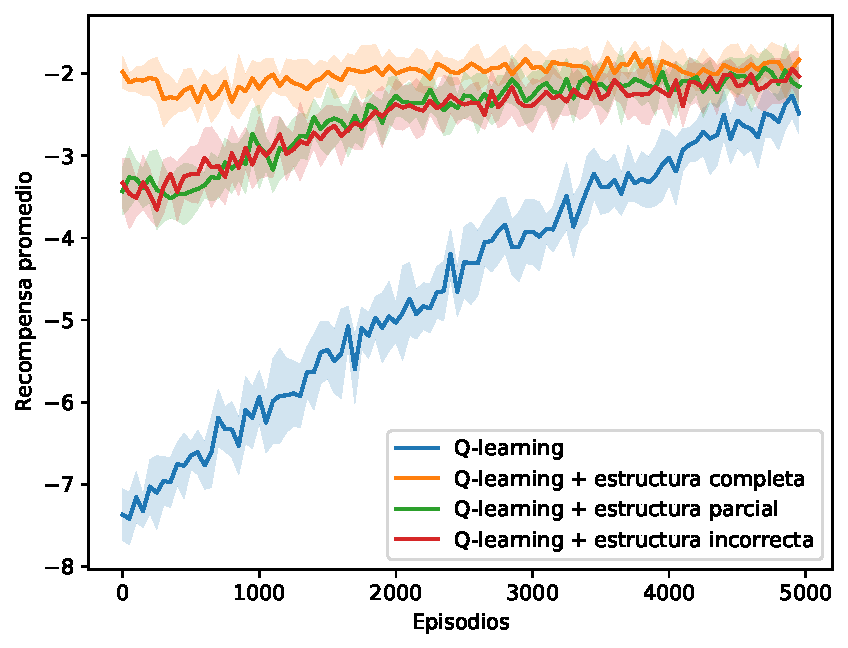
\includegraphics[width=.32\linewidth]{Chapter5/Figs/deltaexp/deterministic_low_025_one_to_one_N_5_experiments_10_episodes_5000_eps_18750.pdf}&
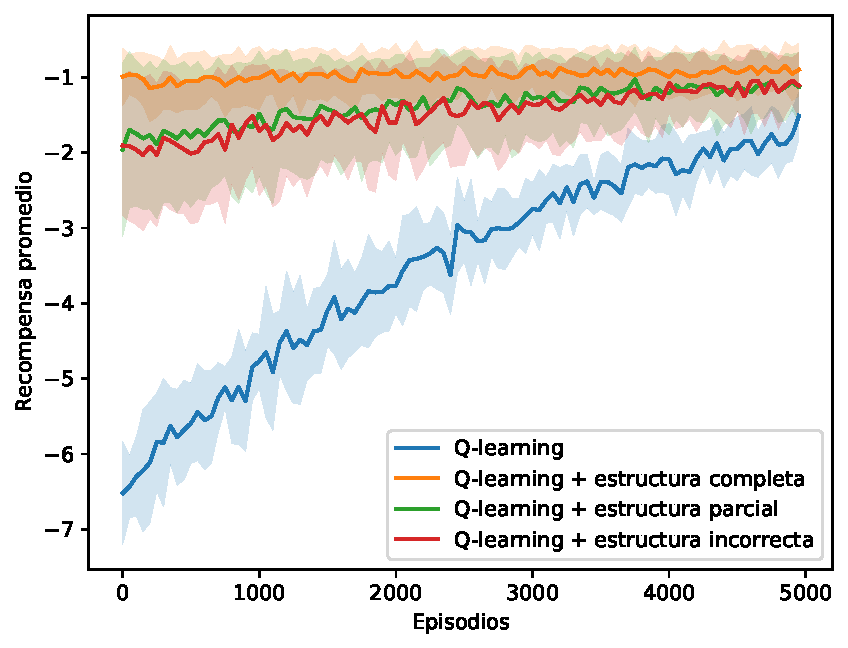
\includegraphics[width=.32\linewidth]{Chapter5/Figs/deltaexp/deterministic_low_025_one_to_many_N_5_experiments_10_episodes_5000_eps_18750.pdf}&
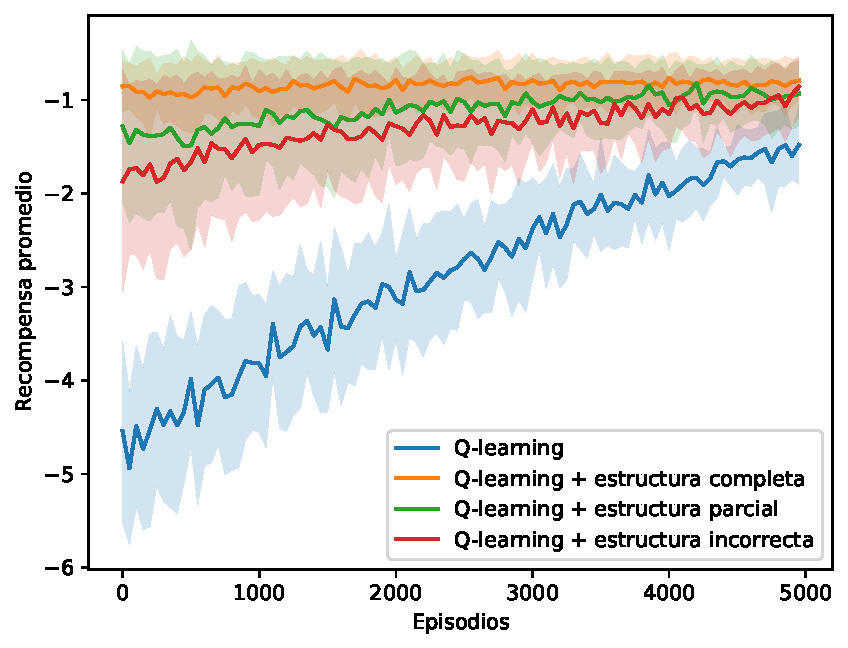
\includegraphics[width=.32\linewidth]{Chapter5/Figs/deltaexp/deterministic_low_025_many_to_one_N_5_experiments_10_episodes_5000_eps_18750.pdf}\\
\rowname{$N=7$}&
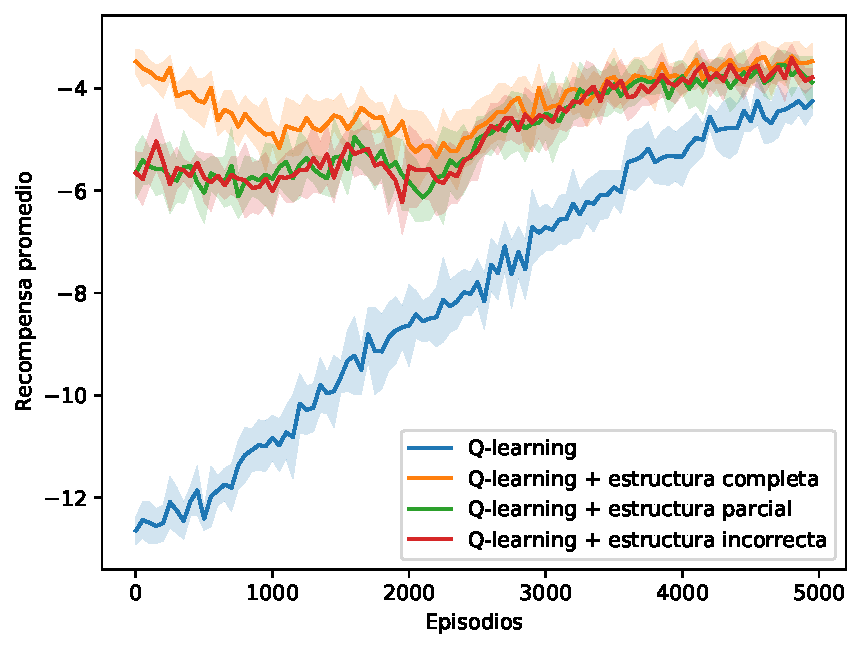
\includegraphics[width=.32\linewidth]{Chapter5/Figs/deltaexp/deterministic_low_025_one_to_one_N_7_experiments_10_episodes_5000_eps_26250.pdf}&
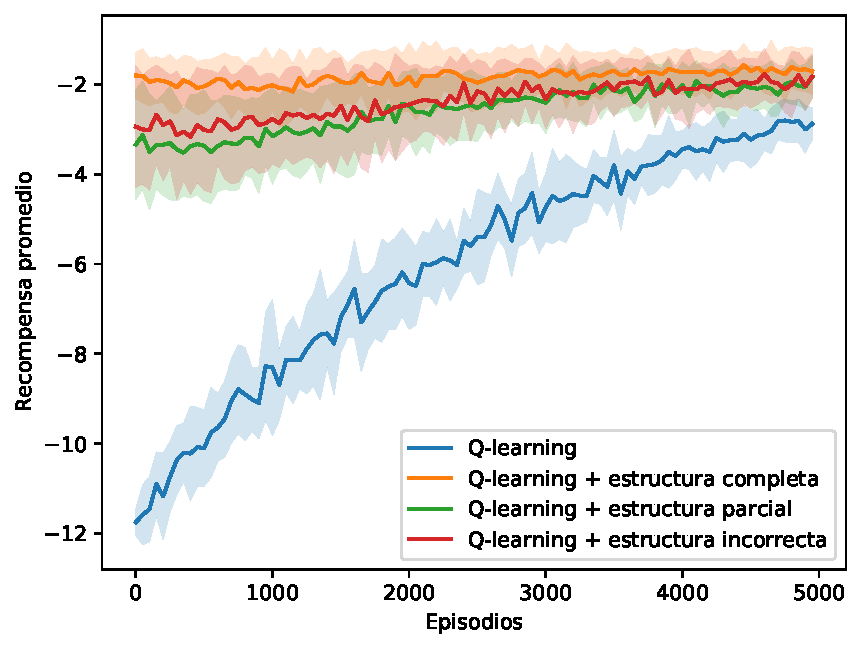
\includegraphics[width=.32\linewidth]{Chapter5/Figs/deltaexp/deterministic_low_025_one_to_many_N_7_experiments_10_episodes_5000_eps_26250.pdf}&
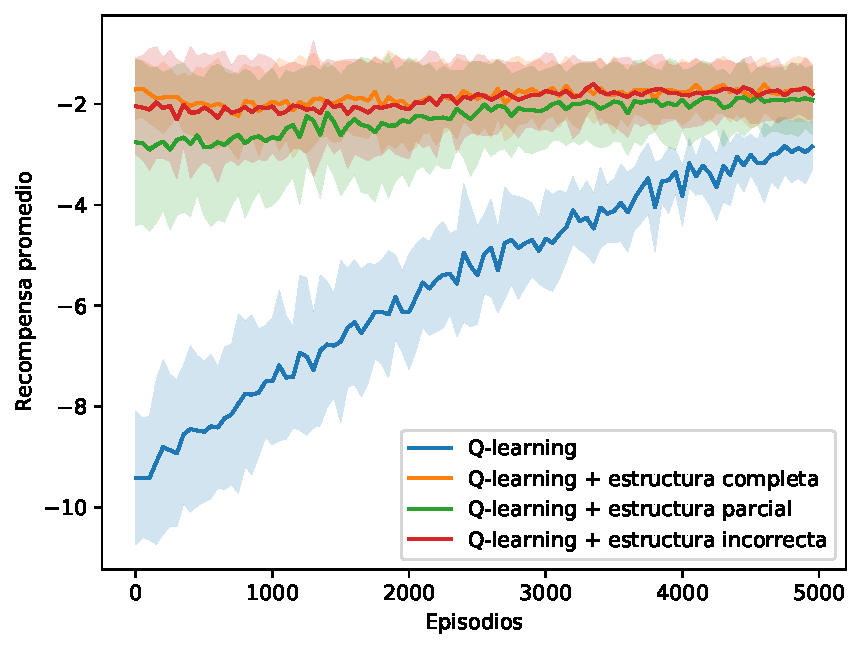
\includegraphics[width=.32\linewidth]{Chapter5/Figs/deltaexp/deterministic_low_025_many_to_one_N_7_experiments_10_episodes_5000_eps_26250.pdf}\\
\rowname{$N = 9$}&
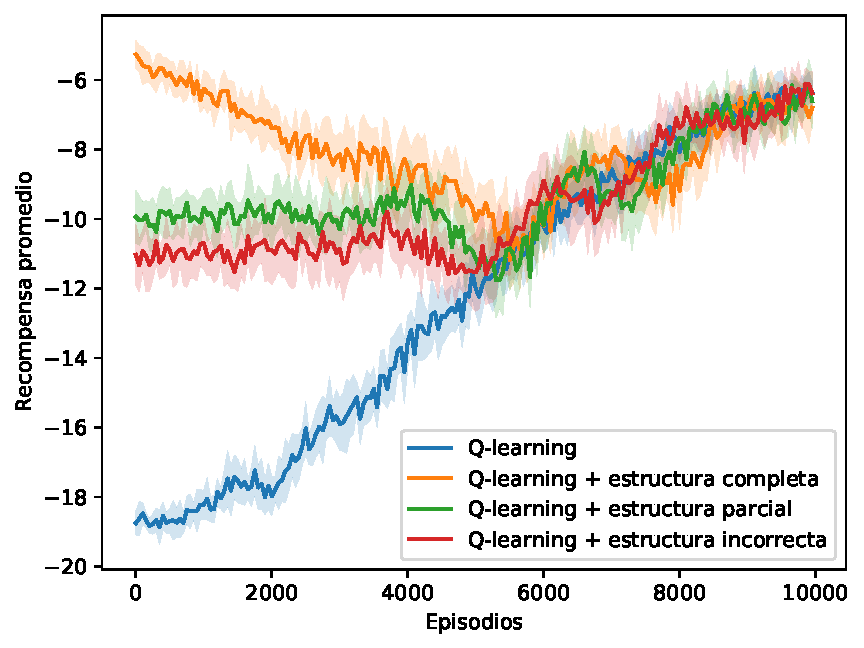
\includegraphics[width=.32\linewidth]{Chapter5/Figs/deltaexp/deterministic_low_025_one_to_one_N_9_experiments_10_episodes_10000_eps_67500.pdf}&
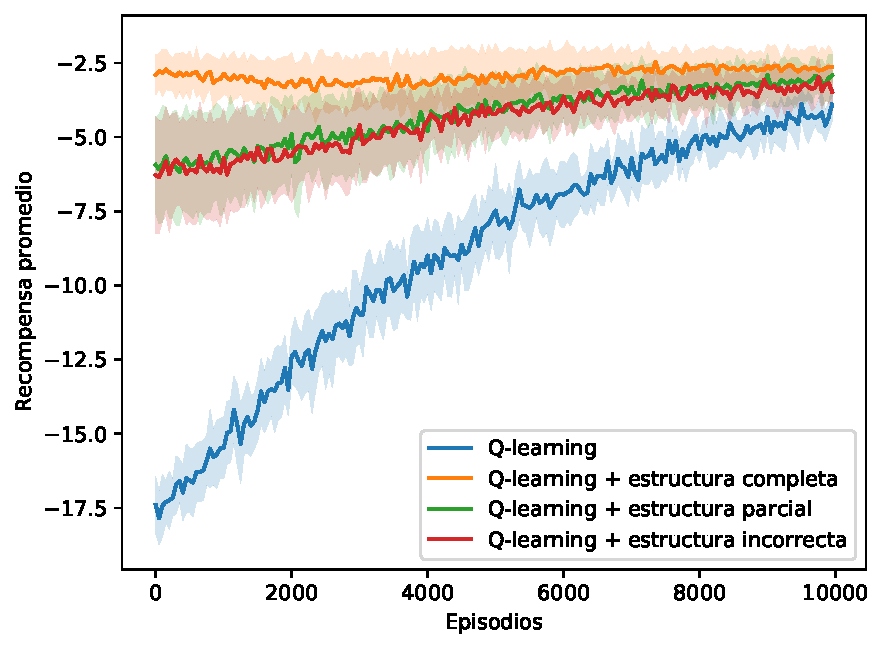
\includegraphics[width=.32\linewidth]{Chapter5/Figs/deltaexp/deterministic_low_025_one_to_many_N_9_experiments_10_episodes_10000_eps_67500.pdf}&
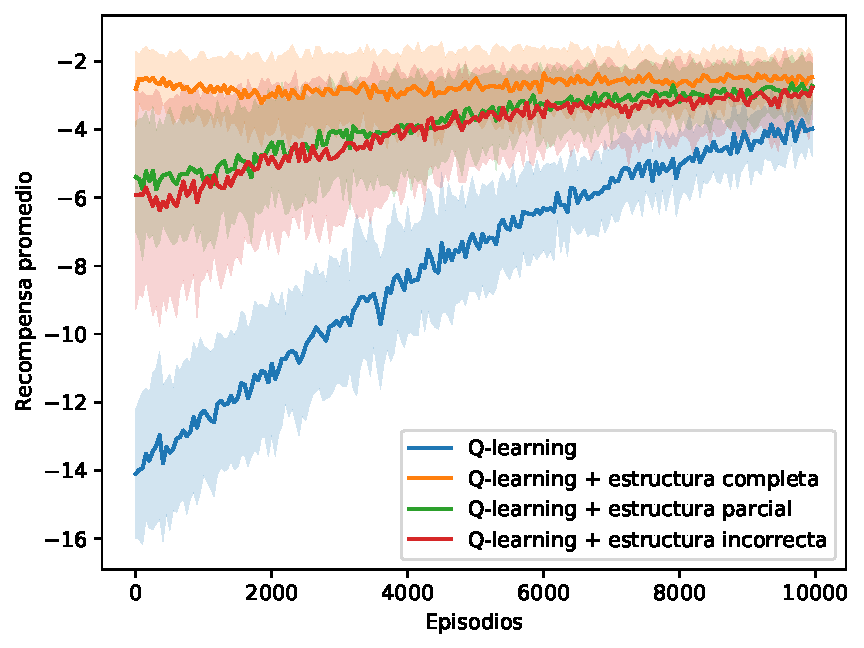
\includegraphics[width=.32\linewidth]{Chapter5/Figs/deltaexp/deterministic_low_025_many_to_one_N_9_experiments_10_episodes_10000_eps_67500.pdf}
\end{tabular}
\caption{Comparación del desempeño para los 4 algoritmos con un nivel de alteración $p_{mod} = 25 \%$ y $\delta = 0.75$ en un ambiente determinista. Las gráficas muestran la medida $average$ y la desviación estándar (región sombreada)  para 10 experimentos con 5000 (para $N = 5, 7$) y 10000 (para $N = 9$) episodios.}
\label{fig:high-epsilon-det}
\end{figure}

\begin{figure}
\settoheight{\tempdima}{\includegraphics[width=.32\linewidth]{example-image-a}}%
\centering\begin{tabular}{@{}c@{ }c@{ }c@{ }c@{}}
&\textbf{Uno-a-uno} & \textbf{Causa común} & \textbf{Efecto común} \\
\rowname{$N = 5$}&
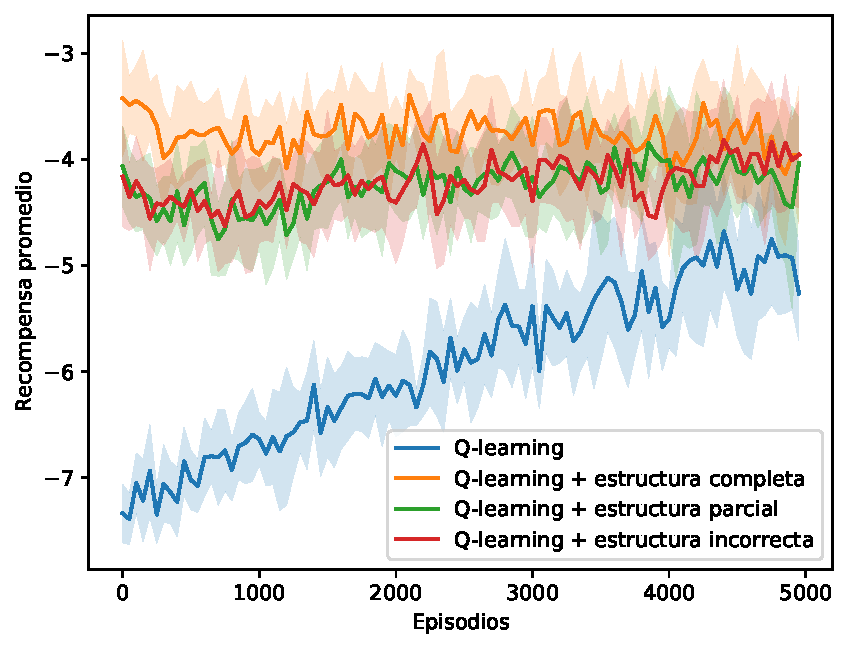
\includegraphics[width=.32\linewidth]{Chapter5/Figs/deltaexp/stochastic_low_025_one_to_one_N_5_experiments_10_episodes_5000_eps_18750.pdf}&
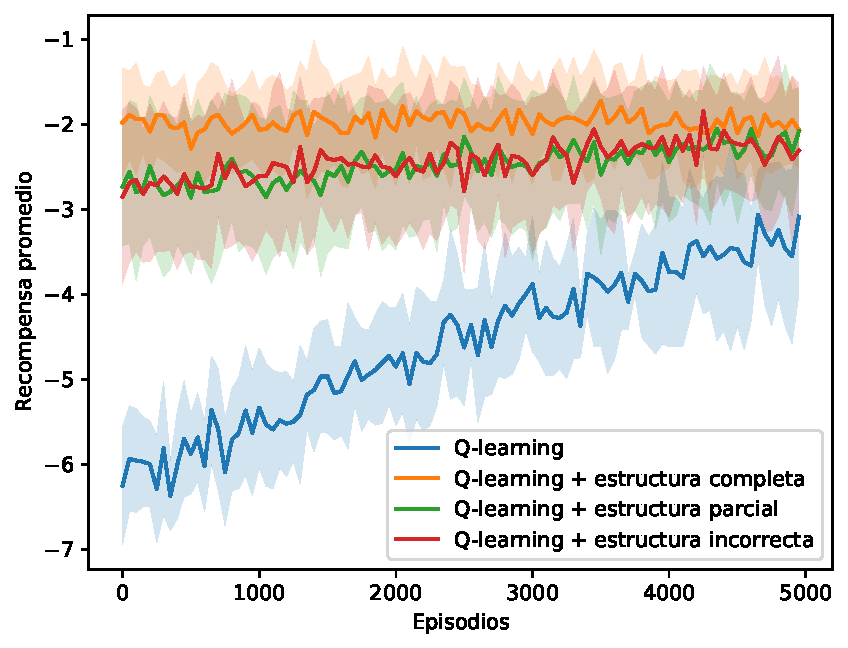
\includegraphics[width=.32\linewidth]{Chapter5/Figs/deltaexp/stochastic_low_025_one_to_many_N_5_experiments_10_episodes_5000_eps_18750.pdf}&
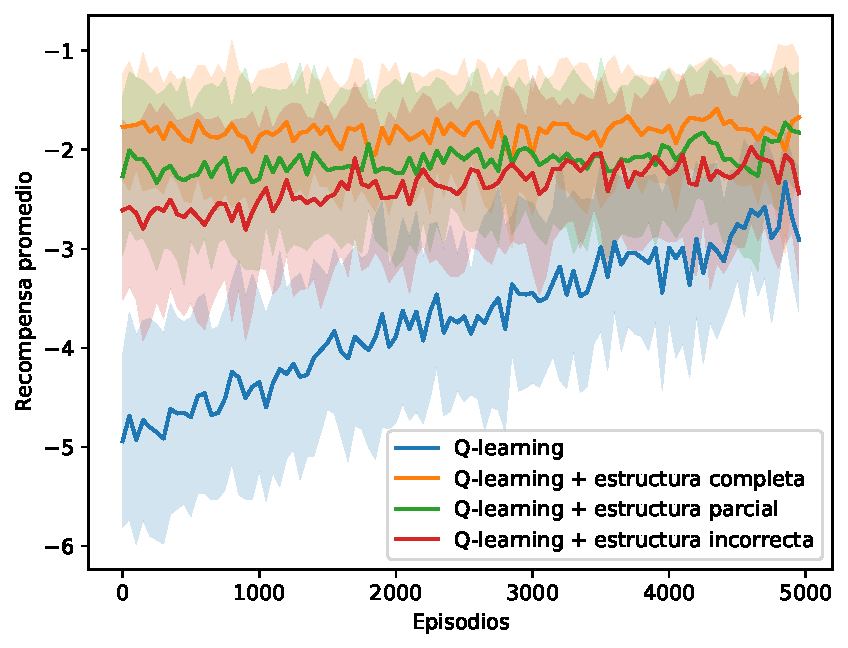
\includegraphics[width=.32\linewidth]{Chapter5/Figs/deltaexp/stochastic_low_025_many_to_one_N_5_experiments_10_episodes_5000_eps_18750.pdf}\\
\rowname{$N=7$}&
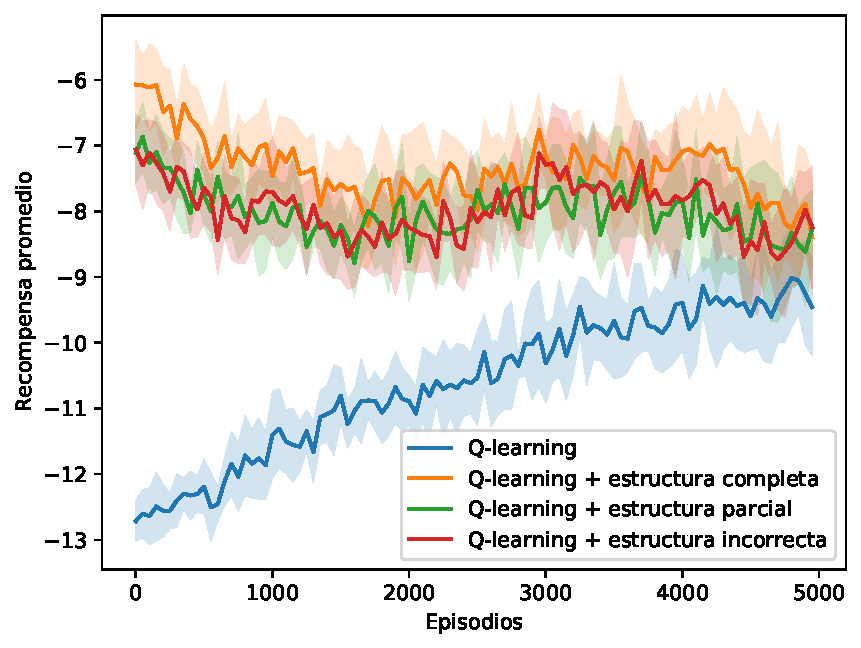
\includegraphics[width=.32\linewidth]{Chapter5/Figs/deltaexp/stochastic_low_025_one_to_one_N_7_experiments_10_episodes_5000_eps_26250.pdf}&
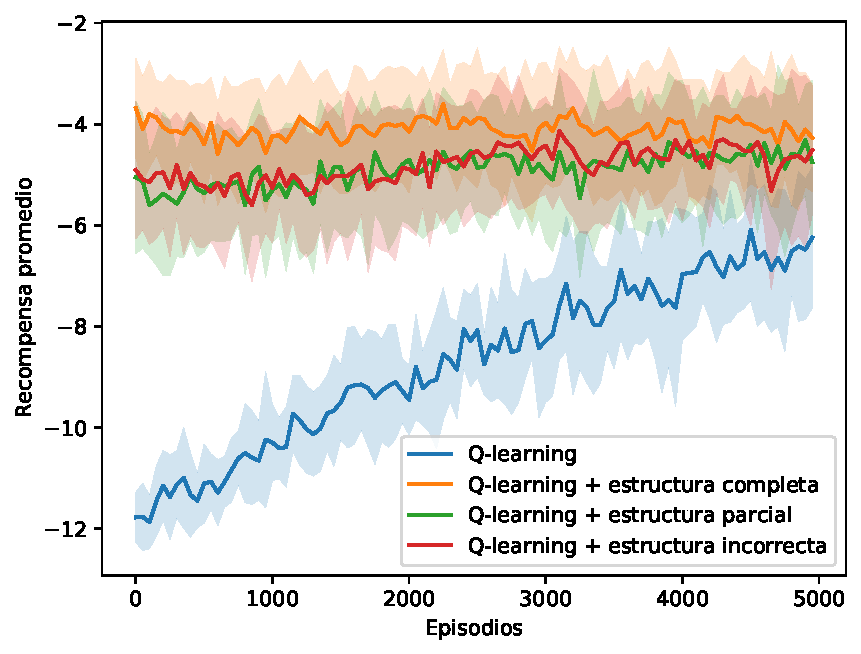
\includegraphics[width=.32\linewidth]{Chapter5/Figs/deltaexp/stochastic_low_025_one_to_many_N_7_experiments_10_episodes_5000_eps_26250.pdf}&
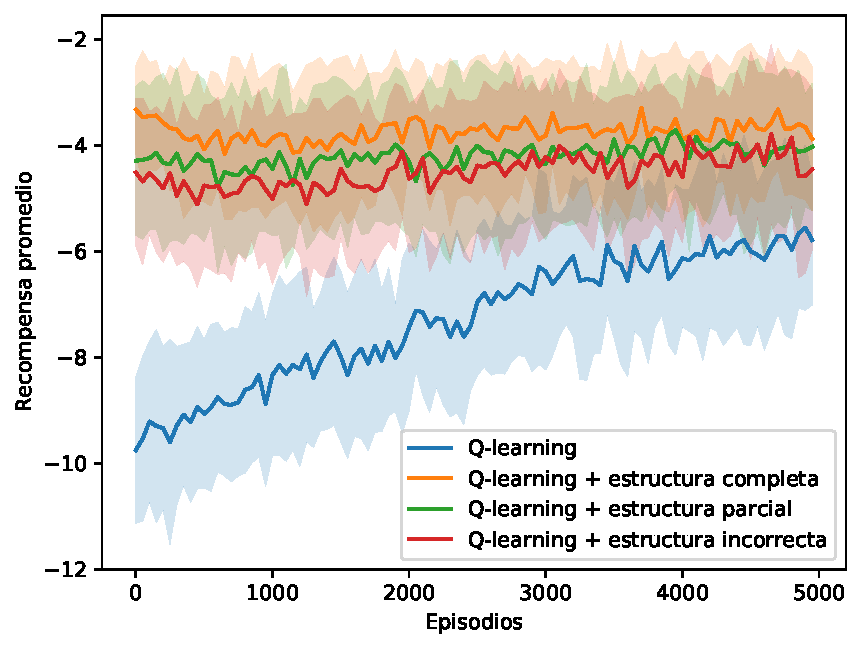
\includegraphics[width=.32\linewidth]{Chapter5/Figs/deltaexp/stochastic_low_025_many_to_one_N_7_experiments_10_episodes_5000_eps_26250.pdf}\\
\rowname{$N = 9$}&
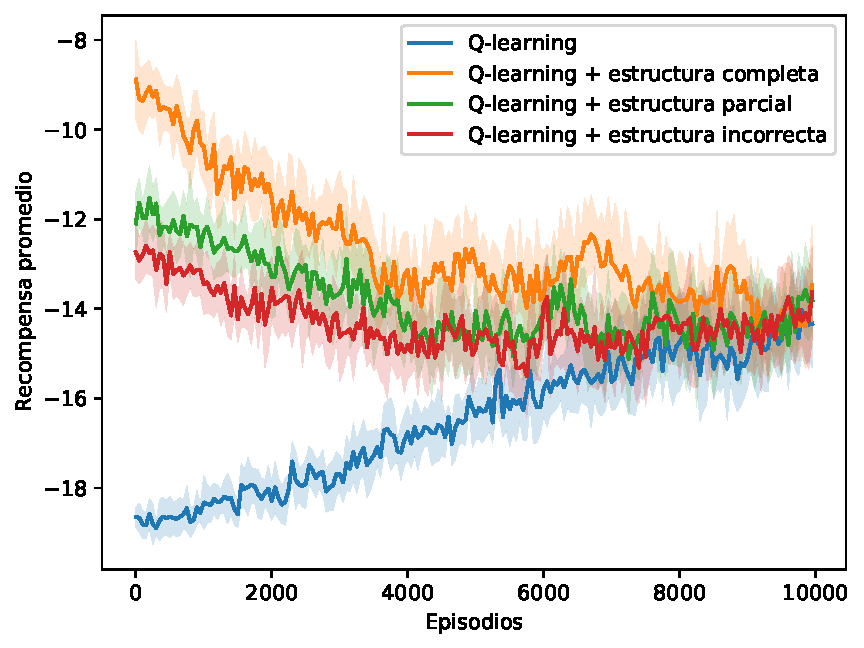
\includegraphics[width=.32\linewidth]{Chapter5/Figs/deltaexp/stochastic_low_025_one_to_one_N_9_experiments_10_episodes_10000_eps_67500.pdf}&
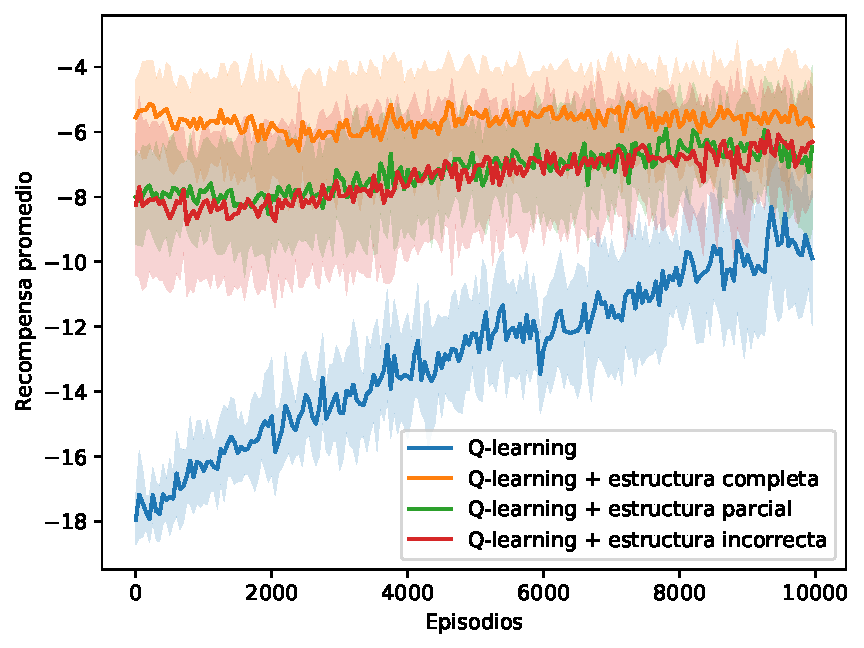
\includegraphics[width=.32\linewidth]{Chapter5/Figs/deltaexp/stochastic_low_025_one_to_many_N_9_experiments_10_episodes_10000_eps_67500.pdf}&
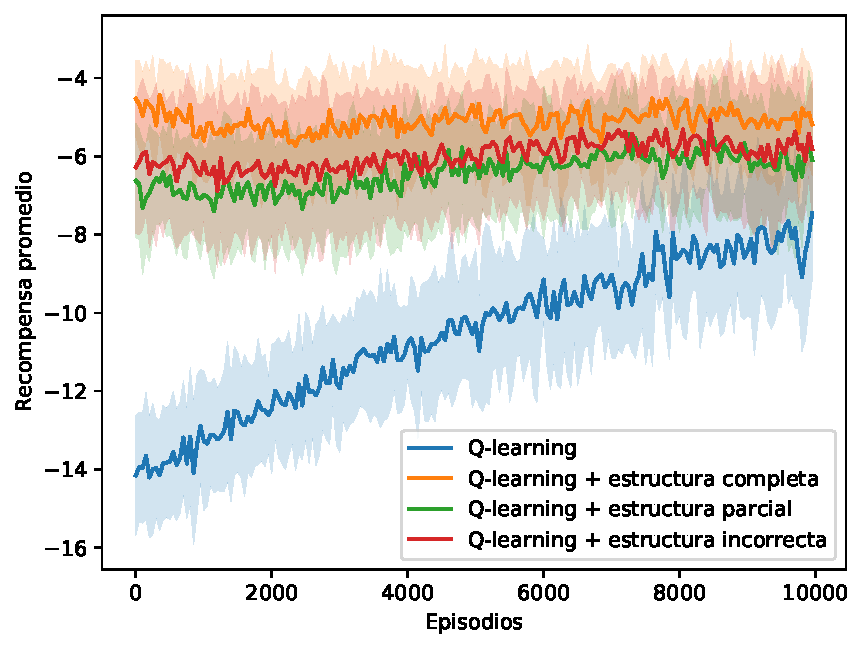
\includegraphics[width=.32\linewidth]{Chapter5/Figs/deltaexp/stochastic_low_025_many_to_one_N_9_experiments_10_episodes_10000_eps_67500.pdf}
\end{tabular}
\caption{Comparación del desempeño para los 4 algoritmos con un nivel de alteración $p_{mod} = 25 \%$ y $\delta = 0.75$ en un ambiente estocástico. Las gráficas muestran la medida $average$ y la desviación estándar (región sombreada) para 10 experimentos con 5000 (para $N = 5, 7$) y 10000 (para $N = 9$) episodios.}
\label{fig:high-epsilon-sto}
\end{figure}

